
\begin{frame}{Case Studies}
MiniBrass wurde für verschiedene Anwendungen eingesetzt:

\vspace*{2ex}

\begin{itemize}
\item \alert<2->{Studenten-Mentoren-Matching}
\item \alert<2->{Prüfungsterminfindung}
\item \alert<2->{Energiefallstudie}
\item Multi-User-Multi-Display
\item Rekonfigurierbare Roboterteams
\item (Rollenallokation im ODP, dzt. nur harte Constraints) 
\end{itemize}
\end{frame}



\begin{frame}[fragile]{Mentor Matching}

\textbf{Ziel}: Teile Mentees (z.B. Studenten) Mentoren zu (z.B. Firmen), sodass
\begin{itemize}
\item Studenten sind sehr zufrieden mit ihren Mentoren
\item Firmen sind mit ihren Mentees ebenfalls zufrieden
\item Zweiseitige Präferenzen
\end{itemize}

\vspace*{2ex}

Bisher klingt das wie ein typisches \emph{Stable Matching}-Problem, aber:

\begin{itemize}
\item Es gibt keine 1:1 Abbildung (Firmen betreuen mehrere Studenten)
\item Zusätzliche Constraints sind vorhanden:
\begin{itemize}
\item[-] Jede Firme betreut zumindest $l$, höchstens aber $u$ Studenten
\item[-] Die Anzahl betreuter Studenten \emph{sollten} ungefähr gleich sein pro Firma (Fairness)
\item[-] Studenten, die eine Firma ``verachten'', sollen nicht gezwungen werden (\emph{harter Ausschluss} von Lösungen)
\end{itemize}
\end{itemize}
\end{frame}


\begin{frame}[fragile]{Mentor Matching: Beispiel}
\begin{center}
\tikzset{onslide/.code args={<#1>#2}{%
  \only<#1>{\pgfkeysalso{#2}}
}}

\tikzstyle{highlight}=[isseorange,ultra thick]
\tikzstyle{highlight2}=[CornflowerBlue,ultra thick,rounded corners]
\tikzstyle{defaultStyle}=[white,ultra thick,rounded corners]

\tikzstyle{impo}=[dashed]
\begin{tikzpicture}[every node/.style={
anchor=base,
%text depth=.5ex,
%text height=2ex,
%minimum height=2ex,
align=center,
rectangle,
text width=2em
}]
\matrix (magic) [nodes in empty cells, ampersand replacement=\&,row sep=0.4cm,column sep=1.5cm]
{
\node[draw,defaultStyle, onslide={<3->{highlight2}}](s1){
\includegraphics[width=\textwidth]{img/businessman.png}}; \& \& \& \node[text width=4em, defaultStyle, draw, onslide={<3->{highlight2}}](c1) {
\includegraphics[width=\textwidth]{img/airplane.png}}; \\
\node(s2){
\includegraphics[width=\textwidth]{img/woman.png}};       \& \& \& \node(c2) {
\includegraphics[width=2\textwidth]{img/logistics.png}}; \\
\node(s3){
\includegraphics[width=\textwidth]{img/man.png}};         \& \& \& \node(c3) {
\includegraphics[width=2\textwidth]{img/enrgy.png}}; \\
\node[defaultStyle, draw, onslide={<3->{highlight2}}](s4){
\includegraphics[width=\textwidth]{img/woman2.png}};      \& \\
};

\draw[onslide={<2->{highlight}}] (s1) -- (c1);
\draw[] (s1) -- (c2);

\draw[onslide={<2->{highlight}}] (s2) -- (c1);
\draw[] (s2) -- (c3);

\draw[onslide={<2->{highlight}}] (s3) -- (c2);

\draw[onslide={<2->{highlight}}] (s4) -- (c3);
\draw[] (s4) -- (c2);
%
%\draw[onslide={<1-2>{highlight}}] (z) -- (3);
%\draw[onslide={<3>{highlight}}] (z) -- (2);
%
%\draw[onslide={<1-2>{highlight}}] (t) -- (2);
%\draw[] (t) -- (1);
%\draw[onslide={<3>{highlight}}] (t) -- (5);
%\draw[] (t) -- (3);
%\draw[] (t) -- (4);
%\draw[onslide={<1>{highlight}}] (u) -- (4);
%\draw[] (u) -- (3);
%\draw[] (u) -- (5);
%\draw[] (u) -- (6);
\end{tikzpicture}
\end{center}
\onslide<2->{Diese \alert{Zuweisung} respektiert die studentischen Präferenzen  (Kanten) \onslide<3->{ignoriert aber die  {\color{CornflowerBlue} Firmenpräferenzen}.}}
\onslide<4->{\tiny OK, es ist nicht wirklich ein \emph{Matching} da Firmen mehr als einen Studenten betreuen \ldots }
\end{frame}

\begin{frame}[fragile]{Mentor Matching: Constraint-Modell}
\begin{lstlisting}
int: n; set of int: STUDENT = 1..n;
int: m; set of int: COMPANY = 1..m;

% assign students to companies
array[STUDENT] of var COMPANY: worksAt;


int: minPerCompany = 1; int: maxPerCompany = 3;
constraint global_cardinality_low_up ( 
           worksAt, [c | c in COMPANY], 
           [minPerCompany | c in COMPANY], 
           [maxPerCompany | c in COMPANY]); 
           
solve 
search pvs_BAB();
\end{lstlisting}
\end{frame}

\begin{frame}[fragile]{Mentor Matching: FMSOFT Instanz}
\begin{lstlisting}
% fmsoft2016.mzn

n = 5; % students
m = 3; % companies

% student names for better readability 
int: raubholz = 1;
int: schraubale = 2;
int: meerfluss = 3; 
int: gleich = 4; 
int: lustig = 5; 

% company names 
int: delphi = 1;
int: cupgainini = 2;
int: youthlab = 3;

\end{lstlisting}

\end{frame}

\begin{frame}[fragile]{Mentor Matching: Präferenzen}
\begin{lstlisting}
PVS: students = new ConstraintRelationships("students") {
   soft-constraint raubholzdelphi: 'worksAt[raubholz] = delphi';
   soft-constraint raubholzyouthlab: 'worksAt[raubholz] = youthlab';
   soft-constraint gleichcupg: 'worksAt[gleich] = cupgainini';
   
   crEdges : '[| mbr.raubholzyouthlab, mbr.raubholzdelphi | 
                 mbr.gleichcupg, mbr.raubholzdelphi |]';
   useSPD: 'true' ;
}; 

PVS: companies = new ConstraintRelationships("companies") {
   soft-constraint delphi_meer: 'worksAt[meerfluss] = delphi';
   soft-constraint delphi_gleich: 'worksAt[gleich] = delphi';
   soft-constraint youthlab: 'worksAt[lustig] = youthlab';
   
   crEdges : '[| mbr.delphi_meer, mbr.delphi_gleich |]';
   useSPD: 'true' ;
}; 

\end{lstlisting}
\end{frame}

\begin{frame}[fragile]{Mentor Matching: Verhalten I}
\begin{lstlisting}
solve ToWeighted(students) lex ToWeighted(companies);
\end{lstlisting}
\begin{Verbatim}[fontsize=\small]
Intermediate solution:worksAt = [3, 2, 1, 1, 1]
Valuations: pen_companies = 1; pen_students = 3
----------
Intermediate solution:worksAt = [1, 2, 3, 1, 1]
Valuations: pen_companies = 2; pen_students = 2
----------
Intermediate solution:worksAt = [1, 3, 1, 2, 1]
Valuations: pen_companies = 3; pen_students = 1
----------
Intermediate solution:worksAt = [1, 1, 1, 2, 3]
Valuations: pen_companies = 2; pen_students = 1
----------
==========
\end{Verbatim}

\end{frame}

\begin{frame}[fragile]{Mentor Matching: Verhalten II}
\begin{lstlisting}
solve ToWeighted(companies) lex ToWeighted(students);
\end{lstlisting}
\begin{Verbatim}[fontsize=\small]
Intermediate solution:worksAt = [3, 2, 1, 1, 1]
Valuations: pen_companies = 1; pen_students = 3
----------
Intermediate solution:worksAt = [2, 1, 1, 1, 3]
Valuations: pen_companies = 0; pen_students = 4
----------
Intermediate solution:worksAt = [1, 2, 1, 1, 3]
Valuations: pen_companies = 0; pen_students = 2
----------
==========
\end{Verbatim}

\end{frame}


\begin{frame}[fragile]{Mentor Matching: WS 15/16}
\begin{itemize}
\item Präferenzen aus E-Mails vom WS 15/16 gesammelt

\begin{parchment}
\begin{verbatim}
"the favorites":
1. JuneDied-Lynx- HumanIT
2. Cupgainini
 
"I could live with that":
3. Seamless-German
4. gsm systems
5. Yiehlke
 
"I think, we won't be happy":
6. APS
7. Delphi Databases
\end{verbatim} 
\end{parchment}
\end{itemize}
\end{frame}

\begin{frame}[fragile]{Mentor Matching: WS 15/16}
\begin{itemize}
\item Priorität zu \alert{Studenten}
\begin{itemize}
\item[-] Was sollen Firmen schon mit unzufriedenen Mentees anfangen?
\end{itemize}
\item Suchraum: 7 Firmen für 16 Studenten $\rightarrow 7^{16} = 3.3233 \cdot 10^{13}$
\vspace*{2ex}
\item Führte zu einem Constraint-Problem mit
\begin{itemize}
\item[-] 77 student. Präferenzen (Soft Constraints) von 16 Studenten
\item[-] insgesamt 114 Soft Constraints (37 Firmenpräferenzen) 
\end{itemize}

\vspace*{2ex}

\item \emph{Bewiesen} optimale Lösung
\begin{itemize}
\item[-] 6 Minuten Lösungszeit
\end{itemize}
\end{itemize}
\end{frame}



\begin{frame}[fragile]{Prüfungstermine}

\textbf{Ziel}: Weise Prüfungstermine an Studenten zu, sodass
\begin{itemize}
\item Jeder Student stimmt seinem Termin zu 
\item Die Anzahl verschiedener Termine wird minimiert (um das Zeitinvestment der Dozenten zu schonen)
\end{itemize}

%\vspace*{2ex}
%\begin{parchment}
\begin{center}

\includegraphics[width=.15\textwidth]{img/voting.png}
\hspace*{4ex}
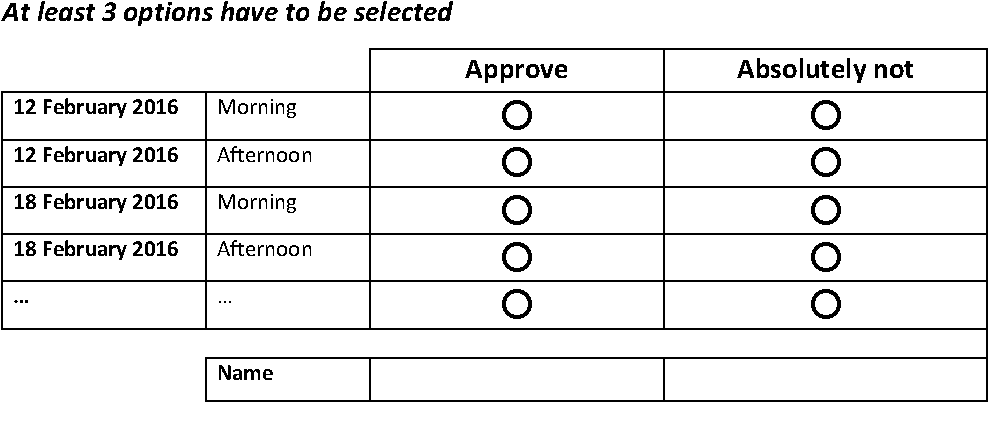
\includegraphics[width=.5\textwidth]{img/Voting.pdf}
\end{center}
%\end{parchment}

\begin{itemize}
\item Kein studentischer Wunsch sollte höher gewichtet werden
\item Prüfungsplan ist eine gemeinsame Entscheidung

\end{itemize}
\end{frame}

\begin{frame}[fragile]{Prüfungstermine: Constraint-Modell}
\begin{lstlisting}
% Exam scheduling example with just a set of 
% approved dates and *impossible* ones
include "globals.mzn";
include "soft_constraints/soft_constraints.mzn";

int: n; set of int: STUDENT = 1..n; 
int: m; set of int: DATE = 1..m;
array[STUDENT] of set of DATE: possibles;
array[STUDENT] of set of DATE: impossibles;

% the actual decisions
array[STUDENT] of var DATE: sd;

int: minPerSlot = 0; int: maxPerSlot = 4;
constraint global_cardinality_low_up(sd % minPerSlot, maxPerSlot
constraint forall(s in STUDENT) (not (sd[s] in impossibles[s])); 
 
\end{lstlisting}
\end{frame}

\begin{frame}[fragile]{Prüfungstermine: Präferenzen}

\begin{lstlisting}
include "../defs.mbr";
PVS: students = new WeightedCsp("students") {
   k: '100';
   soft-constraint raubholz:   'sd[raubholz] in {monday, tuesday}';   
   soft-constraint schraubale: 'sd[schraubale] in {tuesday, wednesday}';
   soft-constraint meerfluss:  'sd[meerfluss] in {tuesday}';
   soft-constraint gleich:   'sd[gleich] in {monday, tuesday}';
   soft-constraint lustig:     'sd[lustig] in {monday, wednesday}';
   % hard by weight (less than bottom)
   soft-constraint lustig-urlaub: 'sd[lustig] != tuesday'
                                :: weights('101'); 
}; 
PVS: teachers = new CostFunctionNetwork("teachers") {
   soft-constraint scheduledDates: 'scheduledDates';
}; 
solve students lex teachers;
\end{lstlisting}
\begin{Verbatim}[fontsize=\small]
Scheduled: [1, 2, 2, 1, 1], Distinct dates: 2
Valuations: mbr_overall_students = 0; mbr_overall_teachers = 2
\end{Verbatim}
\end{frame}


\begin{frame}[fragile]{Prüfungstermine: WS 15/16}

\begin{itemize}
\item Gesammelte Präferenzen von 33 Studenten
\item 12 mögliche Termine (6 Tage, Vormittag und Nachmittag)
\begin{itemize}
\item[-] \emph{Approval}-Menge 
\item[-] \emph{Impossible}-Menge
\end{itemize}

\vspace*{2ex}

\item Aggregiert via Wahl durch Zustimming (\alert{Approval voting}), hat ansprechende wahltheoretische Eigenschaften (Arrow)!
\item Höchstens 4 pro Termin

\item Sofort (61 msec) wurde eine optimale Lösung gefunden, die
\begin{itemize}
\item[-] von \emph{jedem} Student Zustimmung erhält
\item[-] Mit der Minimalanzahl von 9 Terminen auskommt
\end{itemize}
\item Verwendete Strategie (natürlich, \ldots):
\end{itemize}
\begin{lstlisting}
solve students lex teachers;% pro students
\end{lstlisting}
\end{frame}

\begin{frame}[fragile]{Energiefallstudie: Unit Commitment}

\textbf{Ziel}: Weise Kraftwerken Produktion zu, sodass
\begin{itemize}
\item Der Bedarf gedeckt wird
\item Steuerungsvorlieben (ökonomische Leistungsbereiche, \ldots) eingehalten werden
\end{itemize}
\fontsize{8pt}{7.2}\selectfont
\tikzset{
   main node/.style={rectangle,
                     rounded corners,
   					 fill=black!15,
   					 draw,
   					 minimum width=3.5em,
   					 text centered,
                     inner sep=2.5pt,	 
   					 font=\sffamily
   					},
   treestyle/.style={rectangle,fill=black!15,draw,font=\sffamily},
   constraint/.style={circle,fill=black!15,draw,font=\sffamily\small},
   constraint_satisfied/.style = {constraint, fill=white},
   constraint_violated/.style = {constraint, fill=black!25},
}

\begin{figure}[t]
\centering
\begin{tikzpicture}[->,>=stealth',shorten >=1pt,auto,node distance=1.45cm,inner sep=1.5pt,outer sep = 0.0pt, thick] 
%\tikzstyle{every node}=[font=\tiny]
\begin{scope}[xshift=-6.0cm,yshift=-4.0cm]
\node[main node, style={font=\sffamily\footnotesize}] at (0.1,1.5) {\minMaxViolation[1]};
\node[main node, style={font=\sffamily\footnotesize}] at (3.2,1.5) {\minMaxViolation[2]};
\node[main node, style={font=\sffamily\footnotesize}] at (6.3,1.5) {\minMaxViolation[3]};

\draw [rounded corners,dashed,black!45] (-2,2) rectangle (9.0,1);
\node[text width=3cm, anchor=west, right] at (-2.9, 1.5) { \hLevelOrg{1} };
\draw [rounded corners,dashed,black!45] (-2,0.8) rectangle (9.0,-2.65);
\node[text width=4cm, anchor=west, right] at (-2.9, -0.75) { \hLevelOrg{2} };

% bio
\draw [black!85,fill=forestgreen!35] (-1.8,0.6) rectangle (1.8,-2.5);
\node[main node, style={font=\sffamily\footnotesize}] (5) at (0.05,-0.4) {\gasFull};
\node[main node, style={font=\sffamily\footnotesize}] (6) [below left of=5,xshift=5.4] {\ecoSweet};
\node[main node, style={font=\sffamily\footnotesize}] (7) [below right of=5,xshift=-3.1] {\onOff};
%\node[main node, style={font=\sffamily\footnotesize},double] (hardConstraint) [below left of=7,xshift=-3.1,yshift=7] {$\mathsf{maxProd}$};
\node[text width=4cm, anchor=west, left] at (2.3, 0.3) { \textbf{ConstraintRel.:}  $\mathtt{\biogas}$ $(b)$ };
%\node[text width=2cm, anchor=west, left] at (0.4, 0.3) { CR \textsc{TPD} };

% EV
\draw [black!85,fill=black!35] (2.0,0.6) rectangle (5.6,-2.5);
\node[main node, style={font=\sffamily\footnotesize}] (3) at (2.80,-0.4) {\prefBatteryLevel};
\node[main node, style={font=\sffamily\footnotesize}] (4) at (4.58,-0.4)  {\earlyBird};
\node[main node, style={font=\sffamily\footnotesize}] (8) [below right of=3] {\limitBatteryUsage};
\node[text width=3cm, anchor=west, left] at (5.2, 0.3) { \textbf{ConstraintRel.:}  $\mathtt{\ev}$ $(c)$ };
%\node[text width=2cm, anchor=west, left] at (4.3, 0.3) { CR };
%\node[text width=1cm, anchor=east, left] at (5.3, -2.3) { \textsc{SPD} };

% thermal
\draw [black!85,fill=thermicred!25] (5.8,0.6) rectangle (8.8,-2.5);
\draw [rounded corners,dashed,black!45] (5.9,0) rectangle (8.7,-1.3);
\node[text width=4cm, anchor=west, right] at (5.9, 0.2) { \hLevelThermal{1} };
\draw [rounded corners,dashed,black!45] (5.9,-1.8) rectangle (8.7,-2.4);
\node[text width=4cm, anchor=west, right] at (5.9, -1.6) { \hLevelThermal{2} };
\node[main node, style={font=\ttfamily\footnotesize}] (10) at (6.9,-0.4) {\ecoOpt};
\node[main node, node distance=0.85cm, style={font=\sffamily\footnotesize}] (11) at (6.98,-1.0) {\inertia};
\node[main node, node distance=0.85cm, style={font=\sffamily\footnotesize}] (12) at (6.98,-2.1) {\ecoGood};
\node[text width=4cm, anchor=west, right] at (7.1, 0.3) { $\mathtt{\thermal}$ $(d)$ };

\node[text width=2cm, anchor=west, left] at (10, -0.7) { \textbf{CFN:} \\ $\mathtt{h1}$ };

\node[text width=2cm, anchor=west, left] at (10.1, -2.1) { \textbf{CFN:} \\ $\mathtt{h2}$ };

\node[text width=2cm, anchor=west, left] at (10.1, 1.4) { \textbf{CFN:} \\ $\mathtt{orga}$ };

\path[every node/.style={font=\sffamily\tiny}]
  (8) edge node [right] {} (3)
  (8) edge node [right] {} (4)
  (6) edge node [right] {} (5)
  (7) edge node [right] {} (5)
;
\end{scope}

% \begin{scope}[xshift=-0.2cm,yshift=-0.9cm]
% \node[text width=9cm,left] at (0.0, 0.0) {%
% \begin{itemize}[itemsep=2pt]
%   \item something interesting
% \end{itemize}
% };
% \end{scope}

\end{tikzpicture}
%\caption{Case study depicting individual and organizational preference specifications in context.}
\label{fig:preferencesCaseStudy}
\end{figure}
  



%%% Local Variables:
%%% mode: LaTeX
%%% mode: TeX-PDF
%%% mode: TeX-source-correlate
%%% TeX-master: "../quality-quantity-soft-constraints.tex"
%%% End:


\end{frame}


\begin{frame}[fragile]{Unit Commitment: Constraint-Modell}
\begin{lstlisting}
int: T = 5; set of int: WINDOW = 1..T;
array[WINDOW] of int: demand = [20, 21, 25, 30, 29];

int: P = 3; set of int: PLANTS = 1..P;

array[PLANTS] of int: pMin  = [12, 5, 7];
array[PLANTS] of int: pMax  = [15, 11, 9];

array[WINDOW, PLANTS] of var 0..15: supply; 
constraint forall(p in PLANTS, w in WINDOW) 
     (supply[w,p] in pMin[p]..pMax[p]);

array[WINDOW] of var int: violation = 
    [ abs( sum(p in PLANTS) (supply[w, p]) - demand[w] ) | w in WINDOW];

solve search pvs_BAB();
\end{lstlisting}
\end{frame}

\begin{frame}[fragile]{Prüfungstermine: Präferenzen I}

\begin{lstlisting}
PVS: orga = new CostFunctionNetwork("Orga") {
    soft-constraint vio_1: 'violation[1]';
    soft-constraint vio_2: 'violation[2]';
    soft-constraint vio_3: 'violation[3]';
    isWorstCase: 'true';
};
PVS: biogas = new ConstraintRelationships("biogas") {
   soft-constraint gasFull: 
     'forall(w in WINDOW) (supply[w,biogas] >= 13)';
   soft-constraint ecoSweet: 
     'forall(w in WINDOW) (supply[w,biogas] >= 14)';
   soft-constraint onOff: 
     'forall(w in 1..T-1) ( 
        abs(supply[w,biogas] - supply[w+1,biogas]) <= 1)';
   
   crEdges : '[| mbr.ecoSweet, mbr.gasFull | mbr.onOff, mbr.gasFull |]';
   useSPD: 'true' ;
}; 
\end{lstlisting}
\end{frame}

\begin{frame}[fragile]{Prüfungstermine: Präferenzen II} \small

\begin{lstlisting}
PVS: ev = new ConstraintRelationships("ev") {...}; 

PVS: therm1 = new CostFunctionNetwork("therm1") {
  soft-constraint ecoOpt: 
    'sum(w in WINDOW) ( abs(supply[w,thermal] - 8) )';
  soft-constraint inertia: 
    'sum(w in 1..T-1) ( abs(supply[w,thermal] - supply[w+1,thermal]))';
};

PVS: therm2 = new CostFunctionNetwork("therm2") {
  soft-constraint ecoGood: 
    'sum(w in WINDOW) ( abs(supply[w,3] - 9) )';
};

solve orga lex ( biogas pareto ev pareto  (therm1 lex therm2) );
\end{lstlisting}
$P_{\mathtt{org}_1} \ltimes (P_{\prosumer{\biogas}} \times P_{\prosumer{\ev}} \times (P_{\prosumer{\thermal}}^1 \ltimes P_{\prosumer{\thermal}}^2))$
\end{frame}
